% This is a template of the report proposed used for the fourth mandatory exercise on the HCI course at DIKU 2011.
% The template is an approximately direct translation of the original report produced and published by Rolf Molich, www.dialogdesign.dk
% The template is only partial - only selected portions of the original template is included to show it "works". The rest can be synthesized.
% The template probably contains some redundant definitions or other stuff - Remove, update, improve as you see fit.
%
% This file comes in a zip file called ex6-template-tex.zip. The content of the zip file is:
% ex6-template.tex - The main file.
% ex6.sty - A style file for the frontpage and definitions. Must be included on the tex search path/same dir as ex6-template.tex.
% Pics/ - A directory containing 8 smallish PNG files used for compiling this file.
%
% The template was created by Casper Petersen.

\documentclass[10pt,a4paper]{article}      % Book.cls is also usable
\usepackage[utf8]{inputenc}                % UTF8 encoding
\usepackage[T1]{fontenc}                   % Default fonttype and style
\usepackage[danish]{babel}                 % Danish hyphenation pattern
\usepackage{charter}                       % Font type - Can be removed.
\usepackage{graphicx}                      % For graphics
\usepackage{subfig}                        % For subfigures - Can be removed and replaced with standard figures
%% \usepackage{a4wide}                        % Gives us a bit extra spaces in the margins - Can be removed.
\usepackage{color, colortbl}               % Use to define colors and give tables a colored background
\usepackage{fancyhdr}                      % Fancy headers? Yes please.
\usepackage{ex6}                           % Separate form and function plus ugly tex code
\usepackage{tikz}
\author{Michael Budde, Kasper Passov, Niels Ørbæk Christensen, Claus Skou Nielsen}
\title{Test af brugervenlighed af www.faarupsommerland.dk}
\renewcommand{\customer}{Fårup Sommerland}
\date{Oktober 2011}

\usepackage{enumitem}
\setitemize{
    itemsep=0pt
}
\setenumerate{
    itemsep=0pt
}
\setdescription{
  font=\normalfont\bfseries,
  style=sameline,
  leftmargin=\parindent,
  itemsep=0pt,
  listparindent=\parindent
}
\newlist{opgaver}{enumerate}{2}
\setlist[opgaver,1]{label=\arabic*.}
\setlist[opgaver,2]{label=\alph*.}


\pagestyle{fancy}
\fancyhead[L]{Test af Fårup Sommerlands websted}
\fancyhead[R]{Oktober 2011}
%\renewcommand{\headrulewidth}{0.4pt}
%\renewcommand{\footrulewidth}{0.4pt}

\begin{document}

\hbadness=10000
\hfuzz=50pt
\maketitle
\newpage
\setcounter{page}{1}

\section*{Drejebog}

\paragraph{Startbetingelser}
\begin{opgaver}
\item Vi vil starte med at give en kort introduktion til deltageren, hvor vi
forklarer at dette er en test af hjemmesiden og ikke af deltageren, og hvordan
en tænke-højt-test foregår.
\item Deltageren skal bruge en Windows-datamat med Internet Explorer 8
installeret.
\item Internet Explorer vil være åbent, på Kongehusets hjemmeside.
\item Deltagerne får opgaverne udleveret på papir, én af gangen.
\end{opgaver}

\paragraph{Indledende spørgsmål}
\begin{opgaver}
\item Har du været i Fårup Sommerland før? Hvis ja, hvor ofte? Og hvad synes du
om det?
\item Har du været lignende steder for nylig? (Sommerland Sjælland, Bakken,
Bonbonland) Hvis ja, hvor ofte? Og hvad synes du om det?
\item I hvilken forbindelse har du sidst været et af disse steder?
\item Kan du beskrive din nærme familie? (antal, køn og alder)
\item Hvor ofte bruger du internettet, og til hvad?
\item Har du brugt Fårup Sommerlands hjemmeside før?
\item Har du brugt nogle af de lignende steders hjemmesider før?
\item Hvad er dine erfaringer med at bestille billetter eller ferieophold på
internettet?
\item I hvillken grad bruger du internettet til at undersøge et sted, før du
køber billet eller ophold?
\end{opgaver}

\newcommand{\note}[1]{\newline {\small\it Note: #1}}
\paragraph{Opgaver}
\begin{opgaver}
\item Find Fårup Sommerlands hjemmeside.

\item {\it Åbent spørgsmål}
    \begin{opgaver}
    \item En af dine venner fortalte for nylig i begejstrede vendinger om et
    besøg i Fårup Sommerland. Hvis du skulle besøge Fårup Sommerland, hvilke
    oplysninger har du brug for? Find disse oplysninger på Fårup Sommerlands
    webside.
    \end{opgaver}

\item {\it Åbningstider/sæson}
    \begin{opgaver}
    \item Du overvejer at tage til Fårup Sommerland. Find ud af hvornår de har
    åbent og bestem en passende dato. Hvad er åbningstiderne på den dag du har
    valgt?
    \note{Åbningstiderne for de forskellige dele af sæsonen findes under menupunktet "Tider og Priser", i bunden af siden.}
    \end{opgaver}

\item {\it Priser}
    \begin{opgaver}
    \item Find billetprisen hvis du skulle tage din nærmeste familie med.
    \note{Billetpriser findes under menupunktet "Tider og Priser"}
    \item Hvor meget koster billetter der også har mad inkluderet?  
    \note{For at finde disse billetter skal man gå ind under menupunktet "Tider og Priser", og vælge "Fårup Inclusive" i menuen i vestre side.}
    \end{opgaver}

\item {\it Bestil billetter}
    \begin{opgaver}
    \item Bestil billetter til Fårup Sommerland for din familie næste weekend.
    \note{Det er pt. ikke muligt at bestille billetter i webshoppen.}
    \end{opgaver}

\item {\it Adresse/rutevejledning}
    \begin{opgaver}
    \item Find Fårup Sommerlands adresse og find ud af hvordan du nemmest
    kommer dertil.
    \note{Findes under "Planlæg dit besøg" -> "Find vej" -> "Kørselsbeskrivelser" -> "Find den korteste rute her" -> brug Kraks ruteplanlægger.}
    \end{opgaver}

\item {\it Sovemuligheder/spisemuligheder}
    \begin{opgaver}
    \item Du har besluttet dig for at dig og din familie gerne vil bruge 2 dage
    i Fårup Sommerland. Find prisen for et ophold med overnatning på et hotel
    startende den 20. december.
    \note{Man skal vælge "Overnatning", udfylde "Bestil din ferie her"-boksen, og så scroll'e ned eller vælge hotel i højre side.}
    \item Du ved et af dine familiemedlemmer elsker pølser, og ikke kan undvære det i en familietur, kan man få pølser i Fårup Sommerland?
    \note{Der er både grill-selv og Fårup-grill.}
    \end{opgaver}

\item {\it Forlystelser/attraktioner}
    \begin{opgaver}
    \item Din nevø vil meget gerne prøve rutsjebanen Lynet i Fårup Sommerland.
    Hvor høj skal man være for at måtte prøve forlystelsen?
    \note{Man skal være 120 cm.}
    \end{opgaver}

\item {\it Find billetter/bedste tilbud}
    \begin{opgaver}
    \item En kollega fra dit arbejde vil tage en
    4-dages tur til Fårup Sommerland med hans kone og to børn. De har selv et
    sommerhus de vil bo i. Hjælp ham med at finde ud af hvad det vil koste.
    \note{Almindelig billetter kan findes under "Tider og Priser". Miniferie-kort ville passe godt, men findes kun under booking og ingen klar pris kan nævnes.}
    \end{opgaver}

\item {\it Se betingelser for ophold}
    \begin{opgaver}
    \item Du vil gerne booke et ophold for en uge på et af hotellerne. Men du
    er ikke sikker på om du kan den dato. Find ud af hvor længe inden opholdsdatoen
    du kan få dine penge tilbage.
    \note{>30 dage inden: 300 kr. gebyr; 30--8 dage inden: 50\% af prisen; <8 dage inden: ingen godtgørelse.}
    \end{opgaver}

\item {\it Se reviews af opholdssteder}
    \begin{opgaver}
    \item Du har hørt fra venner at Blokhus Klit Golf er et godt hotel. Find,
    om muligt, en beskrivelse og bedømmelser af dette hotel.
    \note{Under "Overnatning" -> "Overnatningssteder" -> "Blokhus Klit Golf" -> "Se bedømmelser"}
    \end{opgaver}

\item {\it Booking af ophold}
    \begin{opgaver}
    \item Bestil hotel-overnatning og billetter til weekendturen med din
    familie på dette hotel.
    \item Dit arbejde har spurgt dig om hvornår du kommer hjem fra ferie, og du
    har glemt hvilken slutdato du har givet hotellet. Find slutdatoen på din
    booking.
    \item Du har lånt en campingvogn af en ven, og ønsker at bo i denne under
    jeres ophold. Ændrer din reservation til at i kan bo på en campingplads.
    \item Du har fundet ud af at du havde andre planer den weekend. Annullér
    reservationen eller skift datoen til weekenden efter.
    \note{Ingen af disse opgaver kan løses, da vi ikke har mulighed for at foretage en booking hos Fårup Sommerland}
    \end{opgaver}

\item {\it Sæsonkort}
    \begin{opgaver}
    \item Du har været så glad for Fårup Sommerland at du gerne vil have et
    sæsonkort. Find ud af hvilke goder et sæsonkort giver, og find priser for
    disse.
    \note{For at finde disse billetter skal man gå ind under menupunktet "Tider og Priser", og vælge "Sæsonkort" i menuen i vestre side.}
    \end{opgaver}

\item {\it Diverse}
    \begin{opgaver}
    \item Har Fårup Sommerland nogle ledige stillinger?
    \note{Pt. ingen ledige stillinger.}
    \item Må man medbringe sit eget mad og drikke til Fårup Sommerland?
    \note{Det må man godt.}
    \item Børnene der skal med på turen begynder at blive meget utålmodige, og
    de har brug for noget underholdning. Har Fårup Sommerland noget
    børneunderholdning på hjemmesiden?
    \note{Under "Parken" kan man vælge "Funzone", hvor der er underholdning for børn.}
    \end{opgaver}
\end{opgaver}

\paragraph{Eftersnak}
\begin{opgaver}
\item Hvad var dit indtryk af siden?
\item Nævn 3 gode og 3 dårlige ting ved siden.
\item Var opgaverne realistiske? Nogen af opgaverne du ikke kunne sætte dig ind i?
\item Havde du nemt/svært ved at finde de ting du skulle på siden?
\item Hvad synes du om menu-punkterne og opdelingen af siden?
\item Var du i tvivl om hvor du skulle kigge først for at løse opgaverne, eller fandt du det nemt?
\item Fandt du siden troværdig? Ville du have tiltro til at bruge faarupbooking.dk eller faarupshoppen.dk? Hvad kunne gøre den mere troværdig?
\item Hvad synes du om forsiden?
\item Fandt du forsiden hjælpsom til løsning af opgaverne?
\item Hvad synes du om skov-temaet på siden, og den animerede baggrund?
\item Ville du have lyst til at bruge siden igen?
\item Hvad kunne få dig til at besøge siden regelmæssigt?
\end{opgaver}

\end{document}

\section*{Resumé}
\setcounter{page}{1} % sets the current page number to 32
\addcontentsline{toc}{section}{Resumé}
Kolding Kommune tilbyder information om kommunen på www.koldingkom.dk.
Webstedet blev lanceret i december 2002. DialogDesign  har gennemført en test
af brugervenlighed af webstedet den 12. og 13-03-2003.

\noindent Formålet med testen er at finde og beskrive problemer i dialogen
mellem typiske brugere og Kolding Kommunes websted, samt at foreslå
velgennemprøvede forbedringsforslag som løser de påpegede problemer.\newline

\noindent Testen er foretaget ved at bede otte personer om at løse typiske
opgaver på webstedet under kyndig overvågning. Denne rapport beskriver de
positive forhold og de problemer som testen har afsløret.\newline

\noindent De væsentligste punkter hvor webstedet fungerer godt:
\begin{itemize}
  \item \textbf{Indholdet er godt}\\ Testdeltagerne var imponerede og overraskede over de store mængder nyttigt indhold på webstedet. Sproget er godt, og testdeltagerne fandt ingen sproglige fejl.
  \item \textbf{Navigation}\\ Navigationen fungerer i det store og hele godt. Testdeltagerne udnyttede effektivt samspillet mellem menuen i venstre side og Mere om boksene i højre side.
  \item \textbf{Svartiderne er gode}
\end{itemize}

De væsentligste punkter hvor webstedet kan fungere endnu bedre:
\begin{itemize}
  \item \textbf{Søgefunktionen}\\
  Anbefalinger til forbedring af søgefunktionen:
  \begin{itemize}
    \item Find de 100-200 søgeord som brugerne synes er vigtigst, ved at analysere søgeord. Giv disse søgeord særbehandling, så de altid fører til et ``perfekt'' søgeresultat.
    \item Giv en konstruktiv meddelelse hvis en søgning ikke giver nogen resultater.
    \item Udelad protokoller, mødereferater, intranetsider og lignende fra standard-søgningen.
    \item Vis den sammenhæng hvori søgeordet optræder, for hvert søgeresultat. Fremhæv søgeordet.
  \end{itemize}
  \item \textbf{Integration med Netborger.dk}\\
  Netborger skal integreres bedre med Kolding Kommunes websted. Se afsnit 9.
  \item \textbf{Effektivitet}\\
  Gør genveje og indeks mere synlige. Tilbyd en kort introduktion til webstedet. Se afsnit 3.
\end{itemize}

\noindent Rolf Molich\\
\noindent DialogDesign\\
\noindent April 2003

\newpage
\tableofcontents
\newpage

\section{Kategorier af kommentarer}
Testdeltagernes kommentarer er klassificeret i følgende kategorier:

\begin{table}[!ht]
\centering
\begin{tabular}{p{0.1\textwidth}p{0.8\textwidth}}\hline
& \\
\vspc\good            & Godt. Denne måde at gøre tingene på syntes testdeltagerne godt om. Den kan tjene som forbillede for andre.\\
& \\
\vspc\goodidea        & God idé. Et forslag fra en testdeltager eller testlederen, som kan medføre en væsentlig forbedring af brugeroplevelsen.\\
& \\
\vspc\smallproblem    & Mindre problem. Testdeltagerne studsede et kort øjeblik.\\
& \\
\vspc\seriousproblem  & Alvorligt problem. Problemet forsinkede testdeltagerne i 1-5 minutter, men testdeltagerne kom videre af sig selv. Gav
                        lejlighedsvis anledning til katastrofer.\\
& \\
\vspc\criticalproblem & Kritisk problem. Gav anledning til hyppige katastrofer. En katastrofe er en situation, hvor webstedet ``vandt'' over
                        testdeltagerne, dvs. en situation som forhindrede testdeltagerne i at løse en rimelig arbejdsopgave på webstedet, eller som irriterede testdeltagerne voldsomt.\\\noalign{\smallskip}\hline
\end{tabular}
\caption{Kategori symboler anvendt i denne rapport}
\label{tab:gt}
\end{table}%
\newpage
\section{Forsiden}

\begin{figure}%
\centering
\subfloat[][\textbf{Forsiden på Kolding Kommunes websted}. Nogle testdeltagerne syntes ikke, at denne side lignede en rigtig forside.]{
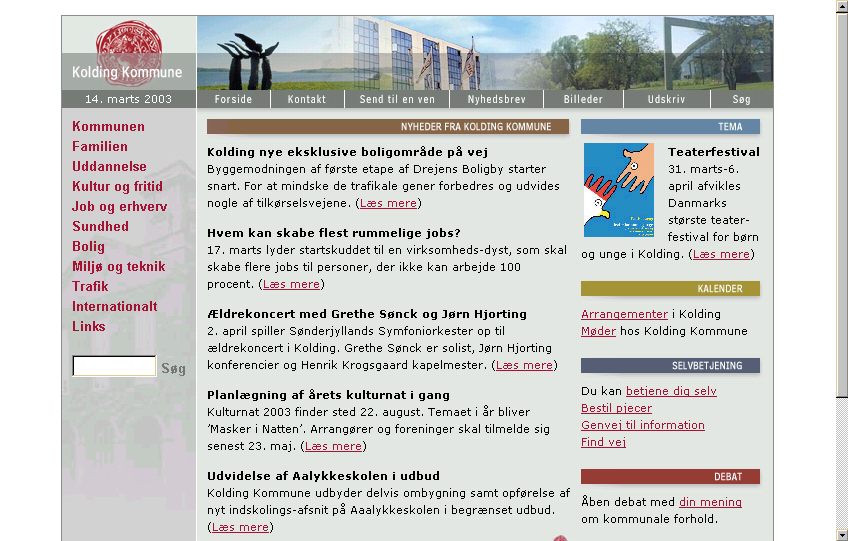
\includegraphics[scale=0.5]{Pics/frontpage}
}%
\qquad
\subfloat[][\textbf{Websiden Kommunen}. Nogle testdeltagere troede, at denne side var webstedets forside, fordi den ``ligner'' en forside, og fordi linket Kommunen i venstremenuen altid er nemt tilgængeligt.]{
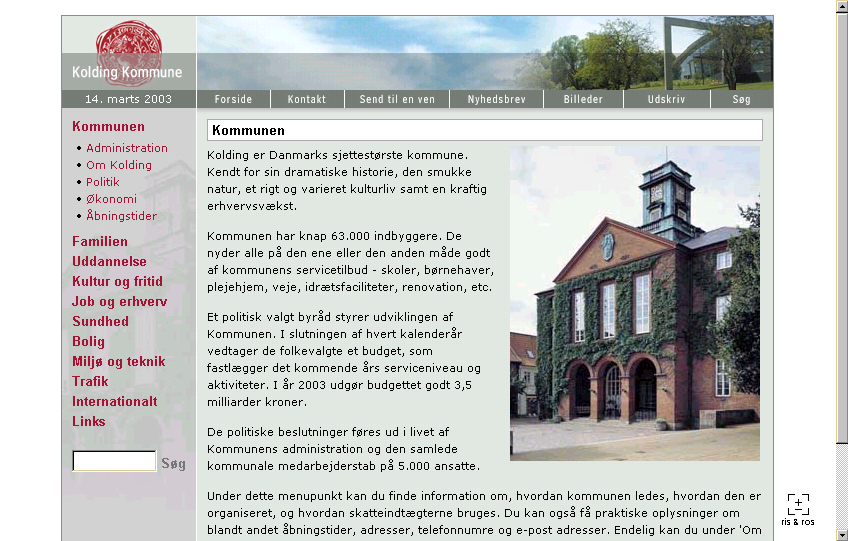
\includegraphics[scale=0.5]{Pics/kommune}
}
\caption{Here are the first two figures of a continued figure.}%
\label{fig:cont}%
\end{figure}

\begin{table}[!ht]
\centering
\begin{tabular}{p{0.1\textwidth}p{0.8\textwidth}}
& \\
\vspc\smallproblem& \textbf{De direkte link til webstedets forside er usynlige}.\\
& Ingen testdeltagere vidste, at de kunne komme til forsiden ved at klikke på kommunens segl i øverste venstre hjørne, selv om dette er en udbredt konvention. Kun nogle få testdeltagere fik øje på linket \emph{Forside} i menulinien øverst i billedet.\newline

Det havde den konsekvens, at mange testdeltagere opfattede siden \emph{Kommunen} som forsiden, fordi linket til denne side er meget synligt (øverst i menuen i venstre side). Nogle testdeltagere brugte Back-knappen for at komme tilbage til forsiden og andre valgte at indtaste URL'en.\\
& \\
\vspc\smallproblem & \textbf{Topmenuen er usynlig}.\\
& Kun nogle få testdeltagere så topmenuen. De testdeltagere, som fik øje på den, kritiserede funktionerne for at være mindre relevante, bortset fra \emph{Forside}.\newline

Testleders kommentar: Topmenuen går i ét med billedfrisen. Separér dem.
Flyt f.eks. følgende funktioner til topmenuen: \emph{Forside}, \emph{Vigtige telefonnumre}, \emph{Åbningstider}, \emph{Søg}, \emph{Genveje}, \emph{Indeks} (dvs. sitemap).
\end{tabular}
\end{table}%


\clearpage
\appendix

\section{Testdeltagernes opgaveløsning}

\begin{table*}[!htp]
\begin{center}
\label{tbl: oversigt}
\small
\begin{tabular}{lccccccccc}
\rowcolor{black}
  \wcolor{Opgave/deltager}     & \wcolor{1}           & \wcolor{2} & \wcolor{3}    & \wcolor{4}       & \wcolor{5} & \wcolor{6}       & \wcolor{7} & \wcolor{8}\\\hline\noalign{\smallskip}
  Find webstedet               & \filler & \good      & \good      & \filler       & \smallproblem    & \good      & \good            & \good\\\cskip
  Gentag tidligere opgave      & \good   & \good      & \good      & \smallproblem & \smallproblem    & \filler    & \filler          & \filler\\\cskip
  Nyt job                      & \filler & \good      & \good      & \filler       & \seriousproblem  & \good      & \good            & \filler\\\cskip
  Rådhus, telf nr., åbningstid & \filler & \good      & \good      & \filler       & \good            & \good      & \good            & \filler\\\cskip
  Oversigt over læger          & \filler & \good      & \good      & \filler       & \criticalproblem & \filler    & \criticalproblem & \filler\\\cskip
\end{tabular}
\caption{Oversigt over testdeltagernes opgaveløsning.}
\end{center}
\end{table*}
\end{document} 
